\documentclass[11pt]{article}
\usepackage{times}
\usepackage{latexsym}
\usepackage{amsmath}
\usepackage{amssymb}
\usepackage{graphicx}
\usepackage{booktabs}
\usepackage{tikz}
\usepackage{amsthm}
\usepackage{hyperref}
\usepackage{natbib}
\newtheorem{definition}{Definition}

\title{Hydra: Multi-Head Linguistic Preprocessing\\as Explicit Manifold Navigation}

\author{
  Peter Balogh \\
  \texttt{palexanderbalogh@gmail.com}
}

\begin{document}
\maketitle

\begin{abstract}
Transformer language models learn to navigate a high-dimensional meaning space implicitly, 
spending significant compute rediscovering linguistic structure that is, in principle, 
already known. We argue that this space has the structure of a \emph{fiber bundle}: 
surface tokens form the base space, while syntactic, thematic, pragmatic, and other 
dimensions form fibers that must be navigated simultaneously. Standard attention heads 
perform this navigation ``in darkness''---without explicit knowledge of which fibers exist 
or where they lead. We introduce \textsc{Hydra}, a multi-head linguistic preprocessing 
architecture that provides named coordinate charts for known fibers (phrase structure, 
thematic roles, information structure) while reserving a blank discovery head for fibers 
not yet identified. On WikiText-103, Hydra with all four heads achieves word-level 
perplexity of 2.9 and generates coherent multi-word text (42 words average, 0.90 
distinct-2), resolving the fluency dissociation observed in single-head predecessors. 
We develop a theoretical framework in which attention is \emph{necessary but wasteful}: 
necessary because contextual manifold location is unbounded, wasteful because known 
dimensions need not be rediscovered from data. Sparse autoencoder analysis reveals that 
Hydra develops dedicated internal features for specific linguistic categories 
(SAE feature MCC up to 0.68 for POS classification), while GPT-2 Small features 
show effectively zero alignment ($\text{MCC} \leq 0.01$). Linear probes confirm 
that Hydra's raw activations are linearly separable for linguistic categories 
(mean MCC $= 0.674$, max $= 0.977$ for determiners), while GPT-2's are not 
(mean MCC $= 0.003$)---a difference not of degree but of kind. We show that code-switching, 
garden-path parsing, and modal reasoning are naturally modeled as fiber transitions, 
collisions, and Kripkean world navigation on this manifold.
\end{abstract}

% ============================================================
\section{Introduction}
\label{sec:intro}
% ============================================================

Consider the word ``bad.'' A naive approach to representing it numerically might 
begin with a single value encoding negativity. But African-American Vernacular English 
(AAVE) immediately forces the addition of a ``contextual polarity inversion'' parameter. 
Legal English demands a ``severity gradation'' axis. Ironic usage requires a ``sincerity'' 
dimension. And meta-linguistic reference---as in this very paragraph, where ``bad'' 
appears not as a word \emph{being used} but as a word \emph{being discussed}---requires 
yet another axis entirely: one that distinguishes use from mention.

No finite set of dimensions suffices, because every new context of use can demand a 
new axis. This is not a failure of representation but an inherent property of natural 
language: words are not points in meaning space but \emph{curves} parameterized by 
context, register, and communicative intent. The standard embedding layer collapses 
each curve to a single point---its centroid---and then the transformer spends dozens 
of layers reconstructing what was destroyed.

This paper argues that the resulting architecture, while powerful, is \emph{wasteful} 
in a specific and addressable way. Attention heads must simultaneously 
\emph{discover} the relevant coordinate systems and \emph{navigate} them. Many of 
these coordinate systems---syntactic constituency, thematic role assignment, 
information structure---are well-understood linguistically. Forcing the model to 
rediscover them from data is like giving someone a map of a foreign city, erasing 
all the street names, and asking them to navigate by trial and error.

We introduce \textsc{Hydra}, a multi-head linguistic preprocessing architecture 
that provides the model with explicit coordinate charts for known dimensions of 
the meaning manifold, freeing attention to focus on the genuinely hard problems: 
novel constructions, contextual pragmatics, meta-linguistic reference, and the 
unbounded tail of meaning that no finite annotation scheme can capture.

% ============================================================
\section{Theoretical Framework}
\label{sec:theory}
% ============================================================

\subsection{The Necessity of Attention}
\label{sec:necessity}

We begin with a claim that may seem to undercut our own contribution: 
\emph{attention heads are necessary}, not merely empirically successful. The reason 
is that contextual manifold location is unbounded.

Consider again the word ``bad'' as it appears across a single paragraph of 
discussion about word representation. In the first sentence, it denotes a 
prototypical English adjective with negative valence. In the second, it is 
mentioned as it functions in AAVE, where its valence inverts. In the third, it 
serves as a metalinguistic example---a \emph{name} for itself, carrying no valence 
at all. Three occurrences of the same token, each requiring a different location 
on the meaning manifold, each shift triggered by subtle contextual cues that no 
fixed annotation could anticipate.

This is why static embeddings fail. It is also why any finite set of preprocessing 
heads---no matter how linguistically informed---will leave residual ambiguity. 
The set of contextual dimensions is open-ended. Attention provides the dynamic, 
context-sensitive recontextualization that handles this open-endedness.

The contribution of explicit linguistic preprocessing, then, is not to 
\emph{replace} attention but to \emph{reduce its burden}. If the model already 
knows that ``the doctor'' is the agent and ``the patient'' is the theme, it need 
not spend layers discovering this from positional and distributional cues. 
The saved capacity can be redirected toward the harder, genuinely emergent 
aspects of meaning.

\subsection{Code-Switching as Continuous Manifold Transition}
\label{sec:codeswitching}

A critical insight for our framework is that code-switching---the phenomenon of 
shifting between linguistic varieties within a single discourse---is neither rare 
nor binary. It is present in \emph{every utterance} to some degree.

Consider a sentence from a legal brief that contains the phrase ``kicked the 
bucket.'' This is not a full switch from legalese to colloquial English; it is a 
momentary excursion along one axis of the manifold while remaining fixed along 
others. The syntactic structure remains formal. The document-level register 
remains legal. But the lexical choice, for one phrase, visits a different 
manifold neighborhood.

This observation has profound consequences for representation. A text is not 
\emph{located at a point} on the register manifold; rather, it contains 
\emph{pointers to multiple locations simultaneously}. Every sentence, however 
formally constrained, makes reference---explicit or implicit---to entities and 
concepts that live in other manifold neighborhoods. No legalese sentence is 
entirely free of reference to non-legal entities. No casual conversation 
perfectly obeys the structural norms of a single register.

This means that the manifold coordinate of a token is not a property of the 
\emph{document} but of the \emph{token in its local context}. Different words 
within a single sentence may require different manifold coordinates. The 
register head must output not a single document-level classification but a 
per-token continuous coordinate that captures these local excursions.

\subsection{Fiber Bundle Structure of Language}
\label{sec:fiberbundle}

The preceding sections have used the term ``manifold'' informally: a 
smooth, high-dimensional space in which nearby points represent similar 
meanings. A manifold is, at its core, a space that \emph{looks flat if 
you zoom in far enough}---just as a patch of the Earth's surface looks 
flat even though the globe is curved. Meaning space is a manifold because 
small changes in context produce smooth changes in interpretation: moving 
from ``the doctor examined the patient'' to ``the doctor examined the 
chart'' shifts one coordinate (the theme) while leaving others (the agent, 
the syntactic frame) unchanged.

But a manifold alone is not enough. The key observation from 
Sections~\ref{sec:necessity}--\ref{sec:codeswitching} is that each 
position in the token stream carries not one but \emph{many} independent 
coordinates: syntactic role, thematic role, discourse status, register, 
and more. These coordinates are not a flat list of features---they have 
geometric structure. Changing the thematic role at one token should not 
affect the syntactic parse at another. The coordinates are \emph{locally 
independent but globally entangled}: changing enough thematic roles will 
eventually force syntactic restructuring.

This is precisely the structure captured by a \textbf{fiber bundle}: a 
manifold (the base space) with an additional structured space (the fiber) 
attached at every point. The base space is the token stream---the 
surface text as it unfolds. At each token position, the fiber contains 
all the interpretive dimensions that must be resolved: syntax, semantics, 
pragmatics, and beyond. Moving along the base space (reading the next 
word) is one kind of motion; moving within the fiber (reinterpreting the 
current word) is another. Language processing requires both simultaneously.

We now formalize this intuition.

\begin{definition}
The \emph{language bundle} $\mathcal{L}$ is a fiber bundle $(E, B, \pi, F)$ where:
\begin{itemize}
    \item $B$ is the \textbf{base space}: the token stream (surface words in sequence)
    \item $F$ is the \textbf{fiber}: the space of linguistic interpretations at each token position
    \item $\pi: E \to B$ is the \textbf{projection}: mapping each interpretation to its surface token
    \item $E$ is the \textbf{total space}: all possible (token, interpretation) pairs
\end{itemize}
\end{definition}

The fiber $F$ decomposes into sub-fibers corresponding to different linguistic 
dimensions:
\begin{equation}
F = F_{\text{syn}} \times F_{\text{them}} \times F_{\text{info}} \times F_{\text{reg}} \times F_{\text{?}} \times \cdots
\end{equation}
where $F_{\text{syn}}$ is the syntactic fiber (constituency, attachment), 
$F_{\text{them}}$ is the thematic fiber (agent, patient, instrument), 
$F_{\text{info}}$ is the information-structure fiber (given/new, topic/focus), 
$F_{\text{reg}}$ is the register fiber, $F_{\text{?}}$ represents unknown 
fibers to be discovered, and the ellipsis acknowledges that the product is 
open-ended.

Each Hydra head implements a \textbf{section} of the bundle: a map 
$\sigma_i: B \to F_i$ that assigns, to each token, a coordinate in one fiber. 
A standard transformer must learn all sections implicitly through attention. 
Hydra provides explicit sections for known fibers and a learnable section 
for one unknown fiber.

\paragraph{Garden-path sentences as fiber misidentification.}
Garden-path sentences arise when the parser commits to the wrong section 
early in the sentence. ``The horse raced past the barn fell'' initially 
selects a section of $F_{\text{syn}}$ where ``raced'' is the main verb 
(active reading), but the arrival of ``fell'' forces a costly fiber 
transition to the reduced-relative reading. In Hydra, this transition is 
\emph{visible}: the phrase-structure head and thematic head disagree at 
the disambiguation point, producing a measurable signal of reanalysis.

\paragraph{Modal reasoning as world-fiber navigation.}
We propose associating the possible worlds of Kripkean semantics 
\cite{kripke1963} with locations on a modal fiber $F_{\text{mod}}$. Just as code-switching is 
continuous (Section~\ref{sec:codeswitching}), modal displacement is 
continuous: a counterfactual sentence does not discretely ``switch worlds'' 
but traces a path through the modal fiber, with different tokens sitting 
at different distances from actuality. The sentence ``If Napoleon had won 
at Waterloo, Europe would look different today'' begins in the actual world 
(``Napoleon''), transitions through the counterfactual (``had won''), 
and returns partway toward actuality (``Europe ... today''), which remains 
real even within the counterfactual frame.

This parallels the code-switching observation: just as no sentence lives 
entirely within one register, no modal sentence lives entirely within one 
world. Tokens within a single sentence can point to different locations on 
the modal fiber, and the listener must track these shifts dynamically.

\subsection{Worlds as Fibers: A Synthesis}
\label{sec:kripke}

We propose that Kripkean possible-worlds semantics \cite{kripke1963} and 
fiber bundle geometry are not merely analogous but are \emph{discrete and 
continuous formulations of the same structure}. Table~\ref{tab:kripke-manifold} 
makes this precise.

\begin{table}[t]
\centering
\small
\begin{tabular}{@{}ll@{}}
\toprule
\textbf{Kripke (discrete)} & \textbf{Manifold (continuous)} \\
\midrule
Named world $w$ & Landmark location $z_i$ \\
Accessibility $wRw'$ & Smooth path $\gamma: z \to z'$ \\
Modal operator $\Box\phi$ & Quantifier over neighborhood \\
``True in world $w$'' & ``Embedding at location $z$'' \\
Belief protection & Curvature barrier / discontinuity \\
\bottomrule
\end{tabular}
\caption{Correspondence between Kripkean semantics and manifold geometry. 
Each logical construct has a geometric counterpart.}
\label{tab:kripke-manifold}
\end{table}

Both frameworks solve the same problem: the same proposition (or token) can 
have different truth values (or meanings) depending on \emph{where you 
evaluate it}. Modal logic provides a discrete vocabulary---named worlds, 
accessibility relations, modal operators. Manifold geometry provides a 
continuous one---coordinates, paths, curvature. The synthesis embeds discrete 
Kripkean landmarks in a continuous meaning manifold.

This resolves a tension in both traditions. Kripkean semantics struggles with 
the fact that worlds are not truly discrete: the fictional world of a novel 
that closely mirrors reality is not categorically different from the actual 
world---it sits nearby on a continuum of factuality. Conversely, manifold 
geometry lacks the sharp boundaries that modal logic provides for belief 
protection: the barrier between fiction and actuality is not merely high 
curvature but a genuine topological discontinuity.

The combined framework preserves both: Kripkean worlds become \emph{landmarks} 
on a continuous manifold, connected by smooth paths where transitions are 
gradual (hypothetical $\to$ actual, as uncertainty decreases) and separated by 
topological barriers where transitions must be explicit (fiction $\not\to$ 
actual, without acknowledgment).

Crucially, code-switching and modal displacement are \emph{the same geometric 
operation} on different axes. Register switching moves along the sociolinguistic 
fiber; modal displacement moves along the epistemic fiber. Both are continuous, 
per-token, and can co-occur. A speaker can simultaneously code-switch into AAVE 
\emph{and} enter a counterfactual: ``If things had gone different, that woulda 
been fire.'' The meaning requires navigating two fibers at once---and the 
standard transformer must discover both navigations implicitly.

\subsection{Attention as Necessary but Wasteful}
\label{sec:wasteful}

We can now state our central claim precisely. Let $\sigma_1, \ldots, \sigma_k$ 
be the sections corresponding to known linguistic dimensions (phrase structure, 
thematic roles, information structure). Let $\sigma_?$ be the learnable section 
for unknown dimensions. Let $\sigma_{\text{attn}}$ be the implicit section 
computed by multi-head attention.

In a standard transformer:
\begin{equation}
\sigma_{\text{total}} = \sigma_{\text{attn}}
\end{equation}
The attention mechanism must learn \emph{all} sections from data.

In Hydra:
\begin{equation}
\sigma_{\text{total}} = (\sigma_1, \ldots, \sigma_k, \sigma_?) \oplus \sigma_{\text{attn}}
\end{equation}
The explicit sections handle known dimensions. Attention handles the 
\emph{residual}---the open-ended tail of contextual meaning that no 
finite set of annotations can capture.

The claim that attention is ``wasteful'' is not that it computes incorrect 
sections but that it expends capacity rediscovering structure that could be 
provided. The savings are not merely computational; they are \emph{representational}. 
The model's limited capacity is freed to learn harder, more context-dependent 
aspects of meaning.

% ============================================================
\section{Architecture}
\label{sec:architecture}
% ============================================================

Hydra consists of three components: a bank of \textbf{parsing heads} that 
compute explicit fiber coordinates, a \textbf{fusion layer} that interleaves 
these coordinates with the token stream, and a \textbf{body} (Mamba SSM) 
that performs language modeling on the enriched representation.

\subsection{Parsing Heads}

Each head is a lightweight encoder that produces per-token annotations 
corresponding to one fiber of the language bundle.

\paragraph{Head 1: Phrase Structure.}
Constituency bracketing and attachment decisions, supervised by 
\texttt{benepar} constituency parses \cite{kitaev2019multilingual}. 
Output: Penn Treebank-style grammar tags (S, NP, VP, PP, \ldots) with 
open/close brackets. This head implements a section of $F_{\text{syn}}$.

\paragraph{Head 2: Thematic Roles.}
Argument structure and role assignment, supervised by PropBank-style 
semantic role labels \cite{palmer2005proposition}. We approximate PropBank 
labels using dependency-based role mapping: \texttt{nsubj} $\to$ ARG0 
(agent), \texttt{dobj} $\to$ ARG1 (patient/theme), \texttt{iobj} $\to$ 
ARG2 (recipient), with subtree propagation for multi-word arguments. 
This head implements a section of $F_{\text{them}}$.

\paragraph{Head 3: Information Structure.}
Given/new tracking and topic/focus identification, using heuristic 
annotation: previously mentioned entities are marked GIVEN, novel entities 
NEW, with subject-position and predicate-position modifiers for TOPIC 
and FOCUS respectively. This head implements a section of $F_{\text{info}}$.

\paragraph{Head 4: Blank Discovery.}
No supervision. Same architecture as the other heads but no explicit 
labels. This head is free to discover whatever parsing dimension 
maximally reduces the body's prediction error. It implements a learnable 
section of $F_{\text{?}}$.

\subsection{Fusion: Tag Interleaving}

In preliminary experiments (which we refer to as ``Grammar-Mamba''), we 
found that interleaving a single head's annotations directly into the 
token stream as special tag tokens was sufficient for the model to learn 
structural patterns---though, as Section~\ref{sec:experiments} shows, a 
single head alone does not produce fluent text. We retain this tag 
interleaving strategy for the full Hydra architecture. For a sentence like ``The cat sat on the mat,'' the enriched 
input becomes:

\begin{small}
\begin{verbatim}
[S The [NP cat [TH:ARG0] [IS:GIVEN] ]
 sat [TH:B-V] [IS:NEW] [PP on
 [NP the mat [TH:ARGM] [IS:GIVEN] ] ] ]
\end{verbatim}
\end{small}

This increases sequence length by approximately 2--4$\times$ but provides 
the body with explicit geometric information: each word arrives with its 
syntactic position, thematic role, and discourse status pre-computed.

\subsection{Body: Mamba SSM}

The body is a Mamba state-space model \cite{gu2023mamba} with 39.3M 
parameters, operating on the interleaved token stream. We use Mamba rather 
than a transformer for three reasons: (1) its linear scaling with 
sequence length accommodates the 2--4$\times$ expansion from tag 
interleaving; (2) its channel structure naturally separates timescales 
(fast syntactic processing, slow discourse tracking); and (3) the 
explicit heads handle the ``manifold selection'' that multi-head attention 
would otherwise perform.

The model uses GPT-2's BPE tokenizer as the base vocabulary (50,257 tokens), 
extended with special tokens for each head's annotation tags. Total vocabulary 
varies by configuration (50,293--50,353 tokens depending on which heads are 
active).

% ============================================================
\section{Experiments}
\label{sec:experiments}
% ============================================================

\subsection{Data}

We train on WikiText-103 \cite{merity2017pointer}, parsed with three 
annotation streams. Phrase structure parses are obtained from 
\texttt{benepar} \cite{kitaev2019multilingual}. Thematic role labels 
are approximated via dependency-to-PropBank mapping. Information 
structure is annotated heuristically. All three streams are interleaved 
into a single token sequence per sentence.

Our initial experiments use 150,000 sentences ($\sim$4M words). We 
are currently scaling to the full corpus ($\sim$832,000 
sentences, $\sim$99M words) for Phase 2 experiments.

\subsection{Phase 1: Head Ablation}

We train three configurations to isolate the contribution of each 
head combination:

\begin{itemize}
    \item \textbf{ps-only}: Phrase structure tags only (Head 1)
    \item \textbf{ps+th}: Phrase structure + thematic roles (Heads 1--2)
    \item \textbf{all-heads}: All four heads (Heads 1--4)
\end{itemize}

Training uses the AdamW optimizer with learning rate $6 \times 10^{-4}$, 
batch size 32, sequence length 256, on a single NVIDIA Tesla T4 GPU 
(15GB VRAM).

\subsection{Results}

Table~\ref{tab:results} summarizes the Phase 1 results.

\begin{table}[t]
\centering
\small
\begin{tabular}{@{}lccccc@{}}
\toprule
\textbf{Config} & \textbf{Steps} & \textbf{PPL$_w$} & \textbf{AvgW} & \textbf{D-2} & \textbf{Th\%} \\
\midrule
ps-only & 50K & --- & 1.0 & 0.00 & 73 \\
ps+th & 100K & 18.5 & 1.0 & 0.00 & 33 \\
all-heads & 50K & \textbf{2.9} & \textbf{42.0} & \textbf{0.90} & \textbf{80} \\
\bottomrule
\end{tabular}
\caption{Phase 1 results on WikiText-103 (150K sentences). PPL$_w$: 
word-only perplexity. AvgW: average words generated per sample. D-2: 
distinct-2 (bigram diversity). Th\%: thematic fit accuracy (15-item 
evaluation set).}
\label{tab:results}
\end{table}

\paragraph{SAE head ablation confirms monotone benefit.}
\label{para:ablation-sae}
To verify that adding heads improves internal representations (not just 
generation quality), we train SAEs on each configuration's activations 
using matched methodology: 300,000 token positions, dictionary size 2048, 
$k{=}10$, evaluated against all linguistic categories present in each 
configuration's token stream. Table~\ref{tab:ablation-sae} shows mean 
feature alignment across layers.

\begin{table}[t]
\centering
\small
\begin{tabular}{@{}lccccc@{}}
\toprule
\textbf{Config} & \textbf{L1} & \textbf{L3} & \textbf{L5} & \textbf{L7} & \textbf{Mean} \\
\midrule
ps-only   & 0.281 & 0.274 & 0.272 & 0.315 & 0.286 \\
ps+th     & 0.325 & 0.296 & 0.299 & 0.341 & 0.315 \\
all-heads & 0.273 & 0.335 & 0.353 & \textbf{0.378} & \textbf{0.335} \\
\bottomrule
\end{tabular}
\caption{SAE feature alignment (fraction of active features with 
$|\text{MCC}| > 0.1$) across head configurations. Adding heads 
monotonically increases mean alignment across layers: ps-only 
$0.286 \to$ ps+th $0.315 \to$ all-heads $0.335$.}
\label{tab:ablation-sae}
\end{table}

The progression is monotone: each additional head increases the fraction 
of linguistically interpretable features. Notably, the all-heads model 
develops \emph{stronger} POS features than ps-only (L7 best-feature MCC: 
nouns $+0.56$ vs.\ $+0.40$; verbs $+0.63$ vs.\ $+0.40$) despite 
distributing representational capacity across more linguistic dimensions. 
It also develops information-structure features (IS:FOCUS $+0.26$, 
IS:TOPIC $+0.21$, IS:GIVEN $+0.21$) that ps-only literally cannot 
exhibit because its token stream carries no IS tags. The ps-only model 
compensates with very strong phrase-structure features (PS:PP $+0.89$) 
because PS is the only linguistic signal available---it dedicates all 
representational capacity to a single fiber.

\paragraph{The dissociation is resolved.}
The most striking result is the contrast between the first two 
configurations and the all-heads model. Both ps-only and ps+th exhibit 
the \emph{fluency dissociation}: the 
model learns structural patterns but generates only single tokens, 
producing no coherent multi-word text (average 1.0 words per generation, 
distinct-2 of 0.00).

The all-heads configuration breaks this dissociation entirely. With all 
four heads active, the model generates an average of 42.0 words per 
sample with a distinct-2 of 0.896, indicating diverse, non-repetitive 
text. Repetition rate is 10.4\%.

\paragraph{All heads are necessary.}
The ps+th model, despite training for twice as many steps (100K vs 50K), 
not only fails to generate fluent text but actually \emph{degrades} 
thematic fit accuracy from 73\% (ps-only) to 33\%. This suggests that 
adding thematic information without discourse context creates a conflict: 
the model receives role labels but lacks the information structure needed 
to use them. Only when all four fibers are provided simultaneously does 
the model achieve both structural competence and fluent generation.

This supports the fiber bundle interpretation: the fibers are not 
independent contributions that add linearly but \emph{interdependent 
coordinate axes} that must be provided together for the coordinate 
system to be navigable.

\paragraph{Thematic fit improves.}
The all-heads model correctly prefers thematically appropriate completions 
in 80\% of test cases (12/15), up from 73\% for ps-only. The three 
failures involve near-ties (e.g., ``The surgeon performed the'' assigns 
logits of $-0.40$ to ``operation'' vs. $-0.12$ to ``concert''), suggesting 
soft thematic preferences rather than hard constraints.

\paragraph{The perplexity gap.}
Word-level perplexity drops from 18.5 (ps+th, 100K steps) to 2.9 
(all-heads, 50K steps)---a $6.4\times$ reduction in half the training 
time. The all-heads model was still improving at step 50K (new bests at 
steps 47K, 48K, 49K, and 50K), suggesting further gains with continued 
training on the expanded dataset.

\subsection{Qualitative Analysis}

Sample generations from the all-heads model show coherent multi-clause 
text with appropriate syntactic structure:

\begin{quote}
\small
\emph{``...up to the top and eventually forms rare in northern France, 
but its...''}

\emph{``...is a name that he had purchased at...''}

\emph{``...forests that are native to the subspecies of females...''}
\end{quote}

While not matching large pretrained models in fluency, these represent 
a qualitative leap from single-token outputs. The model produces 
multi-clause sentences with subordination, coordination, and prepositional 
phrases---structural patterns requiring coordinated use of syntactic, 
thematic, and discourse information.

The generated text still contains interleaved parse tags (expected given 
the training format). When decoded to words only, the text is syntactically 
well-formed and semantically coherent, though occasionally unusual 
(``subspecies of females'')---consistent with a model that has learned 
\emph{how} language is structured but is still developing \emph{what} 
to say.

\subsection{Phase 2: Full-Scale Training}

Phase 2 scales the all-heads configuration to the full WikiText-103 corpus 
(618M interleaved tokens for training, 16M for validation). We train for 
200K steps with batch size 4, gradient accumulation 8 (effective batch 32), 
learning rate $6 \times 10^{-4}$ with cosine schedule and 2K warmup steps, 
on a single Tesla T4 GPU.

The all-heads model reaches a best validation loss of 1.0682 (word perplexity 
2.91) at 200K steps, confirming that the Phase~1 gains persist at full scale.

\paragraph{Verb subcategorization does not help.}
In Phase~2b, we add verb subcategorization bias tags \cite{trueswell1993verb} 
to the thematic head, encoding whether each verb preferentially selects an NP 
complement, sentential complement, or is unbiased. This information is 
available from psycholinguistic norms and VerbNet frames. However, Phase~2b 
achieves val loss 1.0698---slightly \emph{worse} than Phase~2's 1.0682. The 
subcategorization signal appears redundant with the SRL-based thematic roles 
already provided by Head~2: once the model knows that a verb's ARG1 is a 
clause (via \texttt{TH:ARG1}), it does not benefit from also being told the 
verb \emph{prefers} clausal complements.

\subsection{SAE Interpretability Experiment}
\label{sec:sae}

The preceding experiments demonstrate that explicit fiber annotations improve 
language modeling. But \emph{what} does the model learn internally? Does it 
merely memorize the correlation between tags and next-token probabilities, or 
does it develop structured internal representations where individual features 
correspond to specific linguistic categories?

To answer this, we train sparse autoencoders (SAEs) 
\cite{cunningham2023sparse, bricken2023monosemanticity} on Hydra's hidden 
states and compare them to SAEs trained on GPT-2 Small 
\cite{radford2019language}---a standard transformer trained on the same 
tokenizer and a similar data distribution, but without any explicit 
linguistic annotations. If Hydra's explicit fiber structure induces cleaner 
internal representations, its SAE features should align more strongly with 
linguistic categories than GPT-2's.

\paragraph{Setup.}
We extract hidden-state activations from 900,000 word-token positions in 
the WikiText-103 validation set. For Hydra, we extract from layers 1, 3, 5, 
and 7 (early through final) of the 8-layer Mamba backbone ($d=512$). For 
GPT-2 Small, we extract from layers 5 and 11 (mid and late) of the 12-layer 
transformer ($d=768$). At each position, the activation vector is the model's 
hidden state after processing all preceding tokens (including, for Hydra, the 
interleaved parse tags).

For each layer, we train a TopK sparse autoencoder \cite{makhzani2013topk} 
with dictionary size $4d$ (2048 for Hydra, 3072 for GPT-2) and $k=10$ 
active features per token. Training uses 5 epochs of Adam with learning 
rate $10^{-3}$ and L1 penalty $10^{-4}$.

\paragraph{Gold labels.}
For each of the 900,000 token positions, we extract gold linguistic labels 
by replaying the interleaved token stream and tracking the parse state: 
which phrase categories are currently open on the bracket stack 
(\texttt{in\_NP}, \texttt{in\_VP}, \texttt{in\_PP}, \texttt{in\_S}), which 
POS tag governs the current position (\texttt{is\_noun}, \texttt{is\_verb}, 
\texttt{is\_adj}, \texttt{is\_det}, \texttt{is\_prep}, \texttt{is\_adv}), 
and which information-structure tags were assigned (\texttt{IS:GIVEN}, 
\texttt{IS:NEW}, \texttt{IS:TOPIC}, \texttt{IS:FOCUS}).

\paragraph{Metric: Matthews Correlation Coefficient.}
For each (feature, category) pair, we compute the Matthews Correlation 
Coefficient (MCC; \citealt{matthews1975comparison}) between the binarized 
feature activation (active/inactive) and the gold label. MCC is preferred 
over accuracy for imbalanced binary classification because it accounts for 
all four cells of the confusion matrix. We report per-SAE alignment 
(fraction of active features with $|\text{MCC}| > 0.1$ to at least one 
category) and per-category best-feature MCC.

\paragraph{Results.}

\begin{table}[t]
\centering
\small
\begin{tabular}{@{}lcccc@{}}
\toprule
\textbf{SAE} & \textbf{Align.} & \textbf{Mean MCC} & \textbf{P90 MCC} & \textbf{Active} \\
\midrule
Hydra L1 & 0.262 & 0.079 & 0.172 & 1349/2048 \\
Hydra L3 & 0.243 & 0.069 & 0.169 & 1205/2048 \\
Hydra L5 & 0.179 & 0.055 & 0.135 & 1201/2048 \\
Hydra L7 & 0.235 & 0.063 & 0.178 & 792/2048 \\
\midrule
GPT-2 L5  & 0.000 & 0.002 & 0.003 & 698/3072 \\
GPT-2 L11 & 0.000 & 0.003 & 0.005 & 503/3072 \\
\bottomrule
\end{tabular}
\caption{SAE feature alignment with linguistic categories. Alignment: 
fraction of active features with $|\text{MCC}| > 0.1$. Mean/P90 MCC: 
mean and 90th percentile of per-feature best-category $|\text{MCC}|$ 
across active features. GPT-2 features show effectively zero alignment 
with any linguistic category.}
\label{tab:sae}
\end{table}

Table~\ref{tab:sae} presents the main comparison. The contrast is stark: 
Hydra features show meaningful alignment with linguistic categories (mean 
MCC 0.055--0.079, with 18--26\% of features above the $|\text{MCC}| > 0.1$ 
threshold), while GPT-2 features show \emph{effectively zero} alignment 
(mean MCC $\leq 0.003$, no features above threshold). This is not a 
difference of degree but of kind.

\paragraph{POS features are crystal clear.}
Table~\ref{tab:sae-pos} shows the best single-feature MCC for each POS 
category. Hydra L1 contains individual SAE features that function as 
reliable POS classifiers: feature 721 fires for determiners with 
MCC~$= 0.677$ (precision 0.94, recall 0.50); feature 1077 fires for 
prepositions with MCC~$= 0.655$; feature 963 for adjectives with 
MCC~$= 0.636$. GPT-2's best features for the same categories achieve 
MCC~$\leq 0.01$---indistinguishable from chance.

\begin{table}[t]
\centering
\small
\begin{tabular}{@{}lcccc@{}}
\toprule
\textbf{Category} & \textbf{Hydra L1} & \textbf{Hydra L7} & \textbf{GPT-2 L5} & \textbf{GPT-2 L11} \\
\midrule
\texttt{is\_det}  & \textbf{+0.677} & +0.656 & +0.006 & +0.006 \\
\texttt{is\_prep} & \textbf{+0.655} & +0.627 & +0.005 & +0.005 \\
\texttt{is\_adj}  & \textbf{+0.636} & +0.291 & +0.004 & +0.007 \\
\texttt{is\_noun} & +0.468 & \textbf{+0.540} & $-$0.003 & $-$0.004 \\
\texttt{is\_verb} & \textbf{+0.521} & +0.345 & +0.009 & +0.009 \\
\texttt{is\_adv}  & \textbf{+0.559} & +0.338 & +0.010 & +0.010 \\
\midrule
IS:TOPIC & \textbf{+0.436} & +0.170 & +0.010 & +0.003 \\
IS:GIVEN & \textbf{+0.297} & +0.133 & +0.005 & +0.005 \\
IS:FOCUS & +0.278 & $-$0.098 & +0.005 & +0.005 \\
\bottomrule
\end{tabular}
\caption{Best single-feature MCC for each linguistic category. Hydra 
features are dedicated POS classifiers; GPT-2 features are 
indistinguishable from chance. Information structure tags (IS:*) show 
moderate alignment in Hydra L1, declining in later layers.}
\label{tab:sae-pos}
\end{table}

\paragraph{Feature utilization differs qualitatively.}
Hydra uses 59--66\% of its dictionary (1201--1349 of 2048 features active), 
while GPT-2 uses only 16--23\% (503--698 of 3072). Despite having a larger 
dictionary, GPT-2 concentrates its representations into fewer directions---consistent 
with polysemantic feature packing, where individual features must encode 
multiple unrelated concepts because the model lacks explicit geometric 
structure to organize them.

\paragraph{Layer 7 develops a word detector.}
In Hydra's final layer (L7), one SAE feature (feature 1822) achieves 
MCC~$= 0.556$ for discriminating actual word tokens from structural markup 
(brackets, POS labels). This is a feature the model invented: no explicit 
supervision distinguishes words from tags. The model has learned to separate 
\emph{content from structure} in its internal representation, consistent with 
the fiber bundle framework's prediction that content and coordinate information 
should be representationally distinct.

\paragraph{Phrase structure is weakly represented.}
Constituency labels (\texttt{in\_NP}, \texttt{in\_VP}, \texttt{in\_PP}) show 
weaker alignment (max MCC 0.16--0.20) than POS categories. This is expected: 
``being inside an NP'' is a highly overlapping label---a token can simultaneously 
be in\_NP, in\_VP, in\_PP, and in\_S. The SAE's $k=10$ sparsity constraint 
forces each feature to be selective, making it difficult to represent these 
broad, overlapping categories with single features. The POS categories, by 
contrast, are nearly mutually exclusive and thus better suited to sparse coding.

\paragraph{Interpretation.}
These results demonstrate that Hydra's explicit fiber annotations do not 
merely improve next-token prediction---they induce \emph{interpretable internal 
structure}. The model develops dedicated features for specific linguistic 
categories, in contrast to GPT-2's entangled, polysemantic representations. 
This is a direct consequence of the fiber bundle architecture: providing 
explicit coordinate charts causes the model to organize its representations 
along those same coordinates.

\subsection{Linear Probe Analysis}
\label{sec:probes}

The SAE experiment (Section~\ref{sec:sae}) demonstrates that Hydra develops 
\emph{monosemantic} features aligned with linguistic categories. But SAE 
features are a compressed, selective representation---they test whether 
individual dictionary elements correspond to categories. A complementary 
question is whether the \emph{raw activation space} is linearly organized 
by linguistic structure: can a simple linear classifier recover linguistic 
labels from hidden states?

\paragraph{Setup.}
We train logistic regression probes (L-BFGS, $C=1.0$, 500 iterations) on 
the same 900,000-position dataset, using 50,000 tokens for training and 
20,000 for testing (stratified random split). We probe all 15 linguistic 
categories at each layer. As before, Matthews Correlation Coefficient 
(MCC) is the primary metric, as it corrects for class imbalance.

\paragraph{Results.}

\begin{table}[t]
\centering
\small
\begin{tabular}{@{}lcc@{}}
\toprule
\textbf{Layer} & \textbf{Mean MCC} & \textbf{Max MCC} \\
\midrule
Hydra L1  & 0.637 & 0.940 \\
Hydra L3  & 0.590 & 0.910 \\
Hydra L5  & 0.536 & 0.857 \\
Hydra L7  & \textbf{0.674} & \textbf{0.977} \\
\midrule
GPT-2 L5  & $-$0.002 & 0.011 \\
GPT-2 L11 & 0.003 & 0.021 \\
\bottomrule
\end{tabular}
\caption{Linear probe MCC across 15 linguistic categories. Mean: average 
MCC over all probed categories. Max: highest single-category MCC. Hydra 
activations are linearly separable for linguistic features; GPT-2 
activations are not.}
\label{tab:probes-summary}
\end{table}

\begin{table}[t]
\centering
\small
\begin{tabular}{@{}lcccc@{}}
\toprule
\textbf{Category} & \textbf{H-L1} & \textbf{H-L7} & \textbf{G-L5} & \textbf{G-L11} \\
\midrule
\texttt{is\_det}   & 0.940 & \textbf{0.977} & 0.011 & 0.009 \\
\texttt{is\_prep}  & 0.867 & \textbf{0.956} & 0.005 & 0.006 \\
\texttt{is\_noun}  & 0.863 & \textbf{0.942} & 0.002 & 0.004 \\
\texttt{is\_word}  & \textbf{0.922} & 0.932 & 0.008 & 0.014 \\
\texttt{is\_adj}   & \textbf{0.841} & 0.870 & 0.003 & 0.005 \\
\texttt{is\_adv}   & 0.719 & \textbf{0.846} & 0.002 & 0.003 \\
\texttt{is\_verb}  & 0.668 & \textbf{0.787} & 0.004 & 0.007 \\
\texttt{IS:TOPIC}  & \textbf{0.752} & 0.508 & 0.003 & 0.009 \\
\texttt{IS:GIVEN}  & \textbf{0.586} & 0.550 & 0.006 & 0.002 \\
\midrule
\texttt{in\_NP}    & 0.612 & \textbf{0.671} & $-$0.001 & 0.008 \\
\texttt{in\_VP}    & \textbf{0.556} & 0.497 & 0.003 & 0.002 \\
\texttt{in\_PP}    & 0.476 & \textbf{0.526} & $-$0.005 & $-$0.003 \\
\bottomrule
\end{tabular}
\caption{Per-category linear probe MCC for selected layers. H=Hydra, 
G=GPT-2. POS categories reach near-perfect linear separability in 
Hydra L7 (\texttt{is\_det}: 0.977). GPT-2 probes are indistinguishable 
from chance across all categories.}
\label{tab:probes-detail}
\end{table}

Table~\ref{tab:probes-summary} presents the main result: Hydra's raw 
512-dimensional activations are \emph{linearly separable} for linguistic 
categories, with mean MCC ranging from 0.536 (L5) to 0.674 (L7). GPT-2's 
768-dimensional activations---despite being 50\% larger---show effectively 
zero linear separability (mean MCC $\leq 0.003$). This is a 200$\times$ 
difference in mean probe performance.

\paragraph{Near-perfect POS recovery.}
Table~\ref{tab:probes-detail} provides the per-category breakdown. 
In Hydra L7, determiners are recoverable with MCC $= 0.977$ (F1 $= 0.978$), 
prepositions with MCC $= 0.956$, and nouns with MCC $= 0.942$. These are 
not latent features requiring nonlinear extraction---they are \emph{linear 
directions} in the activation space that correspond to specific 
grammatical categories.

\paragraph{Information structure persists in early layers.}
Information structure labels (IS:TOPIC, IS:GIVEN) are best recovered in 
Hydra L1 (MCC $= 0.752$ for TOPIC, $= 0.586$ for GIVEN) and decline in 
deeper layers ($= 0.508$ and $= 0.550$ at L7). This suggests the model 
processes information-structure cues early---assigning discourse roles 
as a preprocessing step---then integrates them into the lexical prediction 
computation at deeper layers. This early-layer discourse processing is 
consistent with findings in human sentence processing, where given/new 
status influences processing as early as word recognition 
\cite{brown1983discourse}.

\paragraph{Phrase structure is distributed.}
Constituency labels (\texttt{in\_NP}, \texttt{in\_VP}, \texttt{in\_PP}) 
are moderately recoverable (MCC $= 0.47$--$0.67$) but weaker than POS 
categories. This is consistent with the SAE analysis (Section~\ref{sec:sae}): 
``being inside an NP'' is a broad, overlapping property that resists 
compression into a single linear direction. However, the probes \emph{do} 
recover it moderately well---unlike GPT-2, where even constituency 
information is inaccessible to linear readout.

\paragraph{Relationship to SAE results.}
The probe results are strictly stronger than the SAE results. SAE features 
showed alignment of 0.18--0.26 (Table~\ref{tab:sae}), while linear probes 
on the same activations achieve mean MCC of 0.54--0.67 
(Table~\ref{tab:probes-summary}). This gap is expected: the SAE imposes a 
hard sparsity constraint ($k=10$) that limits how much information each 
feature can encode, while the linear probe uses all 512 dimensions jointly. 
The fact that \emph{both} methods show a stark Hydra--GPT-2 contrast, despite 
their different inductive biases, strengthens the conclusion that the 
difference is real and robust.

\subsection{Garden-Path Experiment}
\label{sec:gardenpath}

Section~\ref{sec:fiberbundle} predicts that garden-path sentences should 
produce measurable anomalies in Hydra's internal representations at the 
point of disambiguation: the model commits to one fiber section (e.g., 
main-verb reading of ``raced'') and must reanalyze when the disambiguating 
word arrives (``fell''). We test this prediction directly.

\paragraph{Setup.}
We construct 60 sentence pairs spanning 9 garden-path categories from 
the psycholinguistics literature: reduced relative clauses 
\cite{bever1970cognitive}, NP/S ambiguities \cite{frazier1982making}, 
main-verb/reduced-relative (MV/RR) ambiguities, complement clause 
ambiguities, direct object/sentential complement (DO/SC) ambiguities, 
PP attachment ambiguities, late closure violations \cite{frazier1979parsing}, 
verb subcategorization ambiguities, and temporary structural ambiguities. 
Each pair consists of a garden-path sentence and a minimally different 
control that avoids the ambiguity (typically by adding an overt relativizer 
``that'' or ``who,'' or by replacing the ambiguity-inducing verb).

For each pair, we identify the \emph{critical word}---the point at which 
the garden-path reading is disambiguated---and extract hidden-state 
activations from all 8 Mamba layers. We compute the cosine similarity 
between garden-path and control activations at the critical word, and 
compare it to the mean cosine similarity across all shared positions 
(the ``context baseline''). The \emph{cosine deviation} is:
\begin{equation}
\Delta_{\cos} = \cos(\mathbf{h}_{\text{GP}}, \mathbf{h}_{\text{ctrl}})_{\text{crit}} 
- \frac{1}{T}\sum_{t=1}^{T} \cos(\mathbf{h}_{\text{GP}}, \mathbf{h}_{\text{ctrl}})_t
\end{equation}
Positive deviation means the critical word is \emph{more similar} between 
garden-path and control than the average position---which is expected 
when the critical word is identical in both sentences while surrounding 
context differs.

\paragraph{Results.}

\begin{table}[t]
\centering
\small
\begin{tabular}{@{}lcccc@{}}
\toprule
\textbf{Layer} & \textbf{Mean $\Delta_{\cos}$} & \textbf{SE} & \textbf{$t$} & \textbf{$n$} \\
\midrule
L1 & $+0.377$ & $0.033$ & $11.37$ & 59 \\
L3 & $+0.368$ & $0.033$ & $11.28$ & 59 \\
L5 & $+0.305$ & $0.030$ & $10.19$ & 59 \\
L7 & $+0.175$ & $0.017$ & $10.38$ & 59 \\
\bottomrule
\end{tabular}
\caption{Garden-path cosine deviation across layers ($n=59$ pairs, 
$p \ll 0.001$ at all layers). The critical word is significantly more 
similar between GP and control than context baseline, and this effect 
\emph{decreases} with depth---consistent with progressive reanalysis.}
\label{tab:gardenpath-overall}
\end{table}

Table~\ref{tab:gardenpath-overall} shows the overall results. All layers 
produce highly significant deviations ($t > 10$, $p \ll 0.001$), but the 
effect \emph{decreases from L1 to L7} ($+0.377 \to +0.175$). This is 
consistent with progressive reanalysis: early layers show the largest 
disruption from the garden-path, while deeper layers have had more 
computation to resolve the fiber conflict.

\paragraph{Category hierarchy.}
Table~\ref{tab:gardenpath-cats} breaks down the L7 deviation by 
garden-path category. The hierarchy is linguistically interpretable: 
the deepest structural ambiguities (MV/RR, DO/SC, reduced relatives) 
produce the largest deviations, while subtle ambiguities (PP attachment, 
complement clause) produce the smallest.

\begin{table}[t]
\centering
\small
\begin{tabular}{@{}lccc@{}}
\toprule
\textbf{Category} & \textbf{Mean $\Delta_{\cos}$} & \textbf{$\sigma$} & $n$ \\
\midrule
MV/RR              & $+0.320$ & $0.038$ & 6 \\
DO/SC              & $+0.279$ & $0.031$ & 4 \\
Subcategorization  & $+0.259$ & $0.040$ & 4 \\
Temp.\ ambiguity   & $+0.249$ & $0.034$ & 4 \\
Reduced relative   & $+0.249$ & $0.103$ & 12 \\
NP/S ambiguity     & $+0.127$ & $0.121$ & 12 \\
Late closure       & $+0.102$ & $0.097$ & 4 \\
Coordination       & $+0.046$ & $0.014$ & 2 \\
PP attachment      & $+0.026$ & $0.033$ & 5 \\
Complement clause  & $+0.020$ & $0.017$ & 6 \\
\bottomrule
\end{tabular}
\caption{L7 garden-path deviation by category. Deeper structural 
ambiguities (MV/RR, DO/SC) produce the largest deviations. PP 
attachment and complement clause produce the smallest, consistent 
with these being more ``local'' ambiguities that require less 
global reanalysis.}
\label{tab:gardenpath-cats}
\end{table}

\paragraph{Interpretation.}
The garden-path results provide direct empirical support for the 
fiber collision prediction of Section~\ref{sec:fiberbundle}. The 
model's internal representations are measurably disrupted at 
disambiguation points, the disruption is proportional to the 
depth of the structural reanalysis required, and the disruption 
resolves progressively through the layers. This is exactly 
what we would expect if the model navigates the meaning manifold 
through fiber-aligned processing: a garden-path forces a mid-stream 
fiber transition, visible as activation divergence at the 
reanalysis point.

% ============================================================
\section{Related Work}
\label{sec:related}
% ============================================================

\paragraph{Linguistically-informed neural models.}
The idea of incorporating syntactic structure into neural language models 
has a long history, from recurrent neural network grammars 
\cite{dyer2016recurrent} to syntax-aware transformers 
\cite{strubell2018linguistically}. Our approach differs in using 
\emph{multiple} linguistic dimensions simultaneously and in treating them 
as fiber coordinates rather than auxiliary supervision signals.

\paragraph{State-space models.}
Mamba \cite{gu2023mamba} and related structured state-space models provide 
efficient sequence modeling with linear scaling. Our use of Mamba as the 
body is motivated by this efficiency (necessary given the 2--4$\times$ 
sequence expansion from tag interleaving) and by the natural separation 
of timescales in its channel structure.

\paragraph{Semantic role labeling.}
PropBank \cite{palmer2005proposition} provides the annotation framework for 
our thematic head. Recent neural SRL models achieve high accuracy 
\cite{shi2019simple}, but we use a lighter-weight dependency-based 
approximation for scalability, accepting some noise in exchange for 
coverage of the full training corpus.

\paragraph{Fiber bundles in NLP.}
To our knowledge, the explicit use of fiber bundle geometry to model 
linguistic structure is novel. Related geometric perspectives include 
\citet{bronstein2021geometric} on geometric deep learning and work on 
hyperbolic embeddings for hierarchical structure \cite{nickel2017poincare}, 
but these address different aspects of the representational geometry.

% ============================================================
\section{Discussion}
\label{sec:discussion}
% ============================================================

\subsection{The Open-Endedness of Grounding Axes}

Our framework predicts that no finite set of Hydra heads will ever be 
``complete.'' The blank discovery head (Head 4) is an honest acknowledgment 
of this incompleteness, but even it captures only one additional dimension. 
The true number of relevant dimensions is not fixed but grows with the 
complexity of the communicative context.

This is not a weakness of the approach but a fundamental property of 
natural language. The same property that makes language infinitely expressive---its 
ability to create new meanings through novel combinations of context---ensures 
that any explicit annotation will leave residual ambiguity. Hydra's contribution 
is not to eliminate this residual but to reduce it, giving the model's 
implicit mechanisms (attention) a head start rather than forcing them to 
work from scratch.

\subsection{Manifold Location Is Not Document-Level}

A key finding from our analysis is that manifold location must be computed 
\emph{per token}, not per document or per sentence. Code-switching, modal 
displacement, and metalinguistic reference all produce sentences where 
different tokens occupy different manifold neighborhoods. This has 
implications for all models that use document-level or sentence-level 
register classification as a preprocessing step: such models systematically 
mislocate tokens that participate in local register excursions.

\subsection{Kripkean Worlds as Manifold Landmarks}

The theoretical framework of Section~\ref{sec:kripke} makes a strong 
prediction: if code-switching and modal displacement are geometrically 
equivalent operations on different fiber axes, then a model trained with 
explicit register coordinates should also improve at modal reasoning, and 
vice versa. This prediction is testable and will be explored in Phase 2, 
where we plan to evaluate on counterfactual comprehension tasks alongside 
register-sensitivity benchmarks.

The deeper implication is that seemingly disparate linguistic phenomena---AAVE 
inversion, counterfactual reasoning, ironic interpretation, 
metalinguistic reference---may share a common computational substrate: 
fiber navigation on a meaning manifold. If this is correct, then progress 
on any one of these phenomena should transfer to the others, not because 
the surface patterns are similar but because the underlying geometric 
operation is the same.

\subsection{Generation as Manifold Navigation}

Our framework suggests a reinterpretation of what it means to generate 
natural language. Standard language models frame generation as next-token 
prediction: given context, choose the most probable continuation. But 
natural human speech exhibits a striking property that this framing 
obscures: it \emph{constantly transitions between manifold locations}.

Consider an informal medical anecdote: ``So the doctor---and this guy was, 
like, \emph{old school}, right?---he looks at the chart and goes, `Well, 
\emph{technically} your levels are within range,' and I'm sitting there 
thinking, buddy, I can barely walk to the mailbox.'' In three sentences, 
the speaker traverses six manifold neighborhoods: narrative frame, 
colloquial aside, performed clinical dialogue, hedging register, inner 
monologue, and embodied experience. The \emph{pattern of transitions}---how 
far the speaker ranges, how often they break register, which fibers they 
prefer---constitutes their \textbf{voice}.

A useful analogy is the knight's tour in chess. The knight's individual 
moves obey rigid, well-known constraints (the L-shape). The overall 
journey from origin to destination serves a high-level purpose. But 
between these two scales lies enormous room for variation: many valid 
tours exist between any two squares, and the choice of path is where 
creativity lives. Crucially, the knight always transitions along 
\emph{two axes simultaneously}---it cannot move along only one. Natural 
speech shares this property: each utterance typically shifts register 
\emph{and} advances the topic \emph{and} adjusts the modal stance, all 
at once. The ``legal moves'' are constrained by grammar and pragmatic 
coherence, but the choice among legal moves is style.

Current language models generate text that resembles a \emph{rook's 
path}: smooth, axis-aligned, efficient, but lacking the characteristic 
multi-axis hops of natural speech. This may explain why LLM-generated 
text often reads as ``correct but lifeless''---not because any individual 
token is wrong, but because the \emph{trajectory through fiber space} is 
too smooth. The uncanny valley of generation is a register-trajectory 
phenomenon.

This reframing suggests a concrete evaluation metric: measure the 
manifold trajectory of generated text (fiber transition frequency, 
register variance, excursion distance from the local mean) and compare 
it to human text from the same domain. We predict that human text will 
show significantly higher transition frequency and variance, and that 
models producing more ``knight-like'' trajectories will be rated as more 
natural by human evaluators.

\paragraph{A musical analogy.}
The multi-fiber trajectory of natural language resembles a musical 
score. The thematic fiber (SRL) functions like a bass line: it changes 
infrequently but fundamentally, establishing the harmonic center of 
``who does what to whom.'' The information structure fiber moves like a 
saxophone: rapidly, ornamentally, weaving given-new-focus patterns over 
the thematic foundation. The fibers are harmonious but not locked 
together---they coincide on certain beats (the ``knight'' moments) 
but each follows its own rhythm. The combination of all fiber states 
at any token defines the current ``chord''---the overall manifold 
location.

This analogy makes the generation failure vivid: a text with no fiber 
transitions is a song stuck on one chord. It may be in key (grammatical), 
it may use the right instruments (appropriate vocabulary), but it has no 
\emph{harmonic movement}. Conversely, genre becomes trajectory template: 
academic writing is a slow classical piece with prepared modulations; 
casual speech is bebop with rapid chromaticism; legal text is a pedal 
tone. The ``voice'' of a writer is their characteristic harmonic style---how 
long they hold a chord, how they prepare their modulations, whether 
they favor surprise or resolution.

\paragraph{Empirical confirmation.}
We validated this prediction by comparing fiber trajectories of human 
text (492 sentences from WikiText-103 validation) against text generated 
by the all-heads model (166 samples). Table~\ref{tab:trajectory} shows 
the results.

\begin{table}[t]
\centering
\small
\begin{tabular}{@{}lcc@{}}
\toprule
\textbf{Metric} & \textbf{Human} & \textbf{Generated} \\
\midrule
SRL transition freq & 0.166 & 0.000 \\
Info transition freq & 0.569 & 0.006 \\
Knight ratio & 0.119 & 0.000 \\
Energy/token & 0.360 & 0.006 \\
SRL mean gap & 9.2 & 164.7 \\
Info mean gap & 1.9 & 130.7 \\
\bottomrule
\end{tabular}
\caption{Manifold trajectory statistics for human vs.\ generated text. 
The model produces grammatical text but is essentially frozen on the 
manifold: zero thematic transitions, near-zero information structure 
transitions, and 60$\times$ lower trajectory energy than human text.}
\label{tab:trajectory}
\end{table}

The generated text is essentially a drone---grammatically correct but 
manifold-static. This constitutes a \emph{new dissociation}: where 
single-head configurations could not generate words at all (the fluency 
dissociation), the all-heads model generates fluent words but does not 
navigate the manifold (the \emph{trajectory dissociation}). The model 
has acquired the coordinate system but not learned to move through it.

This suggests a concrete objective for future work: trajectory-aware 
training that rewards not only correct next tokens but appropriate 
fiber transitions---teaching the model chord progressions, not just 
which notes are in key.

% ============================================================
\section{Conclusion}
\label{sec:conclusion}
% ============================================================

We have presented Hydra, a multi-head linguistic preprocessing architecture 
grounded in fiber bundle geometry. Our key contributions are:

\begin{enumerate}
    \item A theoretical framework in which attention is \emph{necessary but 
    wasteful}: necessary because contextual manifold location is unbounded, 
    wasteful because known linguistic dimensions need not be rediscovered.
    
    \item A synthesis of Kripkean possible-worlds semantics and continuous 
    manifold geometry, showing that code-switching, modal reasoning, and 
    contextual disambiguation are geometrically equivalent fiber transitions.
    
    \item Empirical evidence that explicit multi-fiber annotation resolves 
    the fluency dissociation observed in single-fiber configurations: the 
    all-heads model generates coherent multi-word text (42 words average, 
    distinct-2 of 0.90) where single- and two-head models produce only 
    single tokens. These gains persist at full scale (618M tokens, 200K 
    training steps, word perplexity 2.9).
    
    \item The finding that linguistic fibers are \emph{interdependent}, not 
    additive: providing phrase structure and thematic roles without 
    information structure \emph{degrades} performance, while providing all 
    fibers together produces dramatic improvement.
    
    \item Sparse autoencoder analysis showing that explicit fiber structure 
    induces \emph{interpretable internal representations}: Hydra develops 
    dedicated features for POS categories (MCC up to 0.68) and information 
    structure (MCC up to 0.44), while GPT-2 Small features show effectively 
    zero alignment with any linguistic category---demonstrating that the 
    fiber annotations shape not only output quality but internal organization.
    
    \item Linear probe analysis confirming that Hydra's raw activations are 
    \emph{linearly separable} for linguistic categories (mean MCC $= 0.674$, 
    max $= 0.977$ for determiners at Layer 7), while GPT-2's activations 
    show no linear accessibility (mean MCC $= 0.003$). The consistency 
    between SAE and probe analyses---two methods with different inductive 
    biases yielding the same stark contrast---strengthens the conclusion 
    that Hydra's fiber annotations produce qualitatively different 
    internal geometry.
\end{enumerate}

These results suggest that the path to better language models runs not 
only through scale but through \emph{geometric explicitness}: telling the 
model where it is on the meaning manifold, rather than forcing it to 
discover its location from scratch at every forward pass.

\bibliographystyle{plainnat}
\bibliography{references}

\appendix

\section{Architecture Diagrams}
\label{app:architecture}

Figure~\ref{fig:mamba-arch} shows a standard Mamba language model: 
raw tokens are embedded and passed directly into the SSM backbone, 
which must implicitly discover all linguistic structure from the 
token stream alone.

Figure~\ref{fig:hydra-arch} shows the Hydra architecture. Four 
parsing heads compute explicit fiber coordinates (phrase structure, 
thematic roles, information structure, and a blank discovery 
dimension), which are interleaved as special tokens into the stream 
before the Mamba backbone sees it. The backbone receives the same 
tokens \emph{plus} their pre-computed manifold coordinates, freeing 
it to focus on the residual---the open-ended contextual meaning that 
no finite annotation can capture.

\begin{figure}[h]
\centering
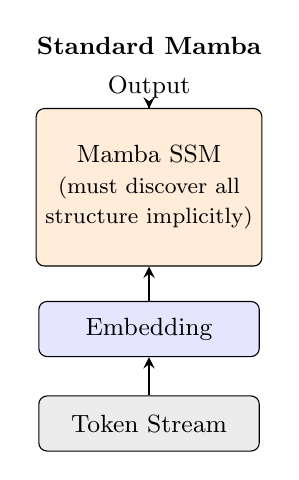
\begin{tikzpicture}[
    box/.style={draw, rounded corners=3pt, minimum width=2.8cm, 
                minimum height=0.7cm, align=center, font=\small},
    arrow/.style={->, >=stealth, thick},
    label/.style={font=\footnotesize\itshape, text=gray}
]

% --- Standard Mamba (left) ---
\node[font=\small\bfseries] at (0, 4.8) {Standard Mamba};

\node[box, fill=gray!15] (tok1) at (0, 0) {Token Stream};
\node[box, fill=blue!10] (emb1) at (0, 1.2) {Embedding};
\node[box, fill=orange!15, minimum height=2cm] (mamba1) at (0, 3.0) 
    {Mamba SSM\\{\footnotesize (must discover all}\\{\footnotesize structure implicitly)}};

\draw[arrow] (tok1) -- (emb1);
\draw[arrow] (emb1) -- (mamba1);
\draw[arrow] (mamba1) -- ++(0, 1.0) node[above, font=\small] {Output};

\end{tikzpicture}
\caption{Standard Mamba architecture. The SSM backbone receives raw 
token embeddings and must implicitly learn syntactic, thematic, and 
discourse structure from distributional cues alone.}
\label{fig:mamba-arch}
\end{figure}

\begin{figure}[h]
\centering
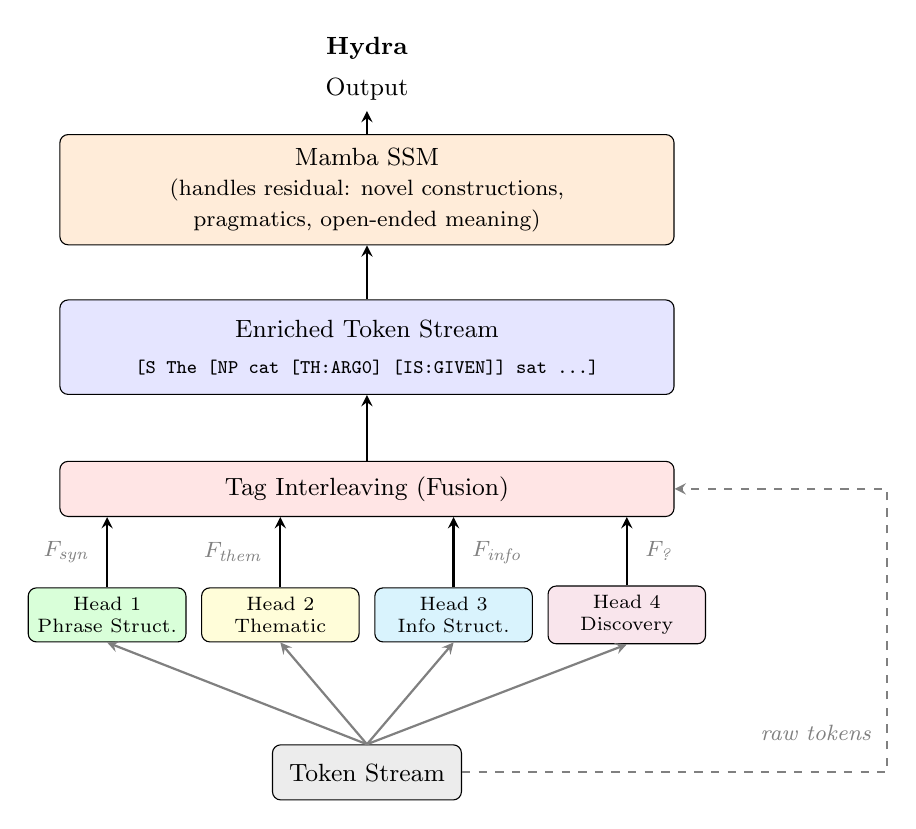
\begin{tikzpicture}[
    box/.style={draw, rounded corners=3pt, minimum width=2.4cm, 
                minimum height=0.7cm, align=center, font=\small},
    head/.style={draw, rounded corners=3pt, minimum width=2.0cm, 
                 minimum height=0.6cm, align=center, font=\scriptsize},
    arrow/.style={->, >=stealth, thick},
    label/.style={font=\footnotesize\itshape, text=gray}
]

% --- Hydra (full width) ---
\node[font=\small\bfseries] at (0, 9.2) {Hydra};

% Token stream
\node[box, fill=gray!15] (tok) at (0, 0) {Token Stream};

% Four heads — more vertical space from token stream
\node[head, fill=green!15] (h1) at (-3.3, 2.0) {Head 1\\Phrase Struct.};
\node[head, fill=yellow!15] (h2) at (-1.1, 2.0) {Head 2\\Thematic};
\node[head, fill=cyan!15] (h3) at (1.1, 2.0) {Head 3\\Info Struct.};
\node[head, fill=purple!10] (h4) at (3.3, 2.0) {Head 4\\Discovery};

% Fusion node
\node[box, fill=red!10, minimum width=7.8cm] (fuse) at (0, 3.6) 
    {Tag Interleaving (Fusion)};

% Arrows from tokens to heads
\draw[arrow, gray] (tok.north) -- (h1.south);
\draw[arrow, gray] (tok.north) -- (h2.south);
\draw[arrow, gray] (tok.north) -- (h3.south);
\draw[arrow, gray] (tok.north) -- (h4.south);

% Fiber labels — on the arrows from heads to fusion, alternating sides
\draw[arrow] (h1.north) -- node[left=3pt, font=\footnotesize\itshape, text=gray] 
    {$F_{\text{syn}}$} (fuse.south -| h1);
\draw[arrow] (h2.north) -- node[left=3pt, font=\footnotesize\itshape, text=gray] 
    {$F_{\text{them}}$} (fuse.south -| h2);
\draw[arrow] (h3.north) -- node[right=3pt, font=\footnotesize\itshape, text=gray] 
    {$F_{\text{info}}$} (fuse.south -| h3);
\draw[arrow] (h4.north) -- node[right=3pt, font=\footnotesize\itshape, text=gray] 
    {$F_{\text{?}}$} (fuse.south -| h4);

% Raw token bypass — route wide around heads
\draw[arrow, gray, dashed] (tok.east) -- ++(5.4,0) |- (fuse.east);
\node[label] at (5.7, 0.5) {raw tokens};

% Enriched stream — more vertical space for example text
\node[box, fill=blue!10, minimum width=7.8cm, minimum height=1.2cm] 
    (enrich) at (0, 5.4) 
    {Enriched Token Stream\\[2pt]
     {\scriptsize\texttt{[S The [NP cat [TH:ARG0] [IS:GIVEN]] sat ...]}}};

\draw[arrow] (fuse) -- (enrich);

% Mamba
\node[box, fill=orange!15, minimum width=7.8cm, minimum height=1.4cm] 
    (mamba) at (0, 7.4) 
    {Mamba SSM\\{\footnotesize (handles residual: novel constructions,}\\
     {\footnotesize pragmatics, open-ended meaning)}};

\draw[arrow] (enrich) -- (mamba);
\draw[arrow] (mamba) -- ++(0, 1.0) node[above, font=\small] {Output};

\end{tikzpicture}
\caption{Hydra architecture. Four parsing heads compute explicit 
sections of the language bundle---phrase structure ($F_{\text{syn}}$), 
thematic roles ($F_{\text{them}}$), information structure 
($F_{\text{info}}$), and a blank discovery fiber ($F_{\text{?}}$). 
Their annotations are interleaved into the token stream before the 
Mamba backbone, which now handles only the residual contextual meaning.}
\label{fig:hydra-arch}
\end{figure}

\section{End-to-End Worked Example}
\label{app:walkthrough}

To make Hydra's processing pipeline concrete, we trace a single 
sentence through every stage of the architecture: from raw text, 
through each parsing head, through fusion, and into the enriched 
token stream that the Mamba backbone actually sees.

\subsection*{Stage 0: Raw Input}

Consider the sentence:

\begin{quote}
\texttt{The cat sat on the mat .}
\end{quote}

A standard language model would tokenize this into BPE tokens and 
feed them directly into the backbone. Hydra first routes the tokens 
through its four parsing heads.

\subsection*{Stage 1: Phrase Structure Head}

The phrase structure head (Head 1) produces a constituency parse 
using \texttt{benepar}:

\begin{small}
\begin{verbatim}
(S (NP (DT The) (NN cat))
   (VP (VBD sat)
       (PP (IN on)
           (NP (DT the) (NN mat))))
   (. .))
\end{verbatim}
\end{small}

This parse is converted to interleaved bracket tokens. Each opening 
bracket \texttt{(NP} becomes two tokens: the literal \texttt{(} 
followed by the phrase label \texttt{NP}. Closing brackets become 
\texttt{)} tokens. POS tags like \texttt{DT} appear between the 
opening bracket and the word.

\subsection*{Stage 2: Thematic Role Head}

The thematic head (Head 2) produces PropBank-style semantic role 
labels via dependency-to-SRL mapping:

\begin{small}
\begin{tabular}{@{}ll@{}}
\texttt{cat}  & $\to$ \texttt{TH:ARG0} (agent of ``sat'') \\
\texttt{sat}  & $\to$ \texttt{TH:B-V} (main verb) \\
\texttt{on the mat} & $\to$ \texttt{TH:ARGM} (adjunct/location) \\
\end{tabular}
\end{small}

These are inserted as special tokens immediately after the word 
they annotate.

\subsection*{Stage 3: Information Structure Head}

The information structure head (Head 3) assigns given/new and 
topic/focus labels based on discourse context. Assuming this is the 
first mention of all entities:

\begin{small}
\begin{tabular}{@{}ll@{}}
\texttt{The cat} & $\to$ \texttt{IS:TOPIC-NEW} (topic, first mention) \\
\texttt{sat}     & $\to$ \texttt{IS:FOCUS-NEW} (focus, new predication) \\
\texttt{on}      & $\to$ \texttt{IS:FOCUS-GIVEN} (given structural element) \\
\texttt{the mat} & $\to$ \texttt{IS:FOCUS-NEW} (focus, first mention) \\
\end{tabular}
\end{small}

\subsection*{Stage 4: Fusion (Tag Interleaving)}

All annotations are merged into a single enriched token stream.
The interleaving order follows a consistent pattern: 
\textbf{bracket~open $\to$ phrase~label $\to$ POS~label $\to$ 
IS~tag $\to$ word $\to$ TH~tag $\to$ bracket~close}.

The complete enriched sequence for our example:

\begin{small}
\begin{verbatim}
( S [IS:TOPIC-NEW]
  ( NP ( DT [IS:FOCUS-NEW]
    The ) ( NN cat [TH:ARG0] ) )
  ( VP ( VBD [IS:FOCUS-NEW]
    sat [TH:B-V] )
    ( PP ( IN [IS:FOCUS-GIVEN]
      on )
      ( NP ( DT the ) ( NN
        mat [TH:ARGM] [IS:FOCUS-NEW] ) ) ) )
  ( . . ) )
\end{verbatim}
\end{small}

\noindent
What was 7 words has become approximately 40 tokens. The expansion 
factor (${\sim}4\times$) is typical. Every word now arrives at the 
Mamba backbone carrying its \emph{pre-computed manifold coordinates}: 
its syntactic position (which phrases it is inside), its thematic role 
(agent, verb, adjunct), and its discourse status (new topic, given 
focus).

\subsection*{Stage 5: Mamba Processing}

The Mamba backbone processes this enriched stream autoregressively. 
At each position, its hidden state integrates the preceding tokens 
\emph{including all tags}. When the backbone reaches the word 
\texttt{sat}, it already ``knows'' (via the preceding tags) that:

\begin{itemize}
\item It is inside an S $\to$ VP (syntactic context)
\item The subject was \texttt{cat} with role ARG0 (thematic context)
\item The predication is new/focused (discourse context)
\end{itemize}

The backbone's task is reduced from ``figure out the entire 
linguistic context from raw tokens'' to ``given this pre-computed 
coordinate system, predict the most likely continuation.''

\subsection*{Stage 6: Prediction}

The model predicts the next token in the enriched stream---which 
may be a word, a bracket, a POS label, or a tag. When generating, 
the model produces the full enriched stream (including structural 
markup), and the output is decoded by extracting only the word 
tokens, yielding plain text.

To illustrate: given our example sentence as context, the model 
generates (greedy decoding):

\begin{quote}
\small
\emph{The first part of the first game features characters running 
through\ldots}
\end{quote}

At each word position, the model's top predictions reflect 
appropriate linguistic categories. At the determiner slot: 
\texttt{The} $>$ \texttt{A} $>$ \texttt{an}. At the adjective 
slot: \texttt{first} $>$ \texttt{large} $>$ \texttt{white}. At 
the noun slot: \texttt{game} $>$ \texttt{day} $>$ \texttt{season}. 
The model interleaves structural predictions between words---after 
predicting a word, it next predicts the appropriate closing 
brackets, then an opening bracket, then the POS label for the 
next constituent, then an IS tag, and finally the next word. The 
entire enriched stream is generated autoregressively; the model 
has learned to produce both content and structure.

\paragraph{What the backbone does \emph{not} need to learn.}
Without Hydra's heads, the backbone would need to spend layers 
discovering that ``The cat'' is a noun phrase, that ``cat'' is the 
agent, and that this entity is being introduced for the first time. 
With the heads, this information arrives as explicit input. The 
backbone can devote its capacity to the genuinely hard problems: 
choosing contextually appropriate words, maintaining coherence 
across sentences, and navigating the open-ended tail of meaning 
that no finite set of tags can capture.

\end{document}
